\documentclass[10pt,a4paper]{article}
\usepackage[utf8]{inputenc}
\usepackage[german]{babel}
\usepackage[T1]{fontenc}
\usepackage{graphicx}
\usepackage{hyperref}
\usepackage{amsmath}
\usepackage{amsfonts}
\usepackage{amssymb}
\usepackage{wrapfig}
\usepackage{multicol}
\usepackage{tikz}
\usepackage{tikz-qtree}
\usepackage[left=2cm,right=2cm,top=2cm,bottom=2cm]{geometry}
\author{Jonas Betzendahl}
\title{Fortgeschrittene Funktionale Programmiernug in Haskell}

\parindent0pt

\begin{document}

\huge \underline{Fortgeschrittene Funktionale Programmiernug in Haskell}\smallskip

\Large
\begin{center}
\textbf{Projekt:} Spielentwicklung in Haskell (Sokoban)\bigskip

\normalsize
\underline{Tutoren:}
Jonas Betzendahl \texttt{(jbetzend@techfak...)},
Stefan Dresselhaus \texttt{(sdressel@techfak...)}
\end{center}
\normalsize

\section*{\underline{Aufgabenstellung:}}

\begin{wrapfigure}{R}{0.35\textwidth}
  \vspace{-30pt}
  \begin{center}
    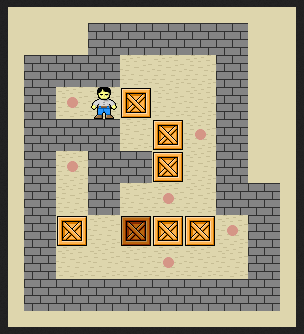
\includegraphics[scale=0.5]{sokoban.png} 
  \end{center}
  \vspace{-15pt}
  \caption{Ein mögliches Sokoban-Level. Credit: \emph{Carloseow (Wikipedia)}}
  \vspace{-90pt}
\end{wrapfigure}

Bei diesem Projekt sollen Sie ein kleines Spiel mit grafischer Oberfläche (GUI) in Haskell schreiben. In Ihrer Implementation soll das Spiel \href{http://en.wikipedia.org/wiki/Sokoban}{Sokoban} spielbar sein, in dem es darum geht, alle Kisten auf markierte Zielpunkte zu schieben (mit nur wenig Platz für Manöver).

\subsection*{Mindestanforderungen:}

Das Spiel muss fehlerfrei spielbar sein (also: Siegbedingungen überprüfen, korrekte Kollisionsabfrage, \dots), bei erfolgreich absolviertem Level automatisch das nächste Laden und einen Counter enthalten, wie viele Züge in diesem Level bereits getätigt wurden.\bigskip

Es sollen mindestens zehn spielbare Level vorliegen, die bei Spielstart aus einer oder mehreren externen Textdateien geladen werden sollen.\\
Diese Dateien sollen auch mit einem Texteditor veränderbar sein, um\\ zum Beispiel zusätzliche Level hinzuzufügen.\bigskip
 
Eine grafische Oberfläche ist Pflicht (Ausgabe auf der Konsole  genügt \emph{nicht}!), die Wahl der GUI-Bibliothek (\texttt{sdl2}, \texttt{gtk2hs}, \dots) steht Ihnen jedoch frei. 

\subsection*{Zusatz:}

Bei besonderer Motivation können außerdem die folgenden Features noch eingebaut werden:
 
\begin{itemize}
\item \textbf{Rückgängig-Funktion:} Ermöglichen Sie es dem Benutzer, seine Züge einen nach dem anderen (bis zum Start des Levels) via Knopf- oder Tastendruck rückgängig zu machen.

\item \textbf{KI zum Lösen:} Gegeben ein beliebiges Level, implementieren Sie eine Funktion, die ermittelt, ob es für dieses Level eine Lösung gibt und welches die kürzeste Abfolge von Zügen ist, die das Level absolviert.

\item \textbf{Levelgenerierung:} Anstelle eine bestimmte Anzahl vorgefertigter Level bereit zu stellen, schreiben Sie einen Algorithmus, der ein zufälliges (lösbares, siehe oben) Level generiert. So kann ein Spielmodus erstellt werden, den man theoretisch ewig weiter spielen könnte.
\end{itemize}

\section*{\underline{Abgabemodalitäten:}}

Eine gültige Abgabe ist ein \texttt{cabal}-Projekt, das fehlerfrei in einer Sandbox installiert werden kann und eine funktionierende ausführbare Datei generiert (Testumgebung ist im Zweifelsfall wie immer das GZI). Bitte reichen Sie Ihre Projekte spätestens bis zum \textbf{Freitag, den 18.09.2015} ein.
Dazu schicken Sie alle Dateien, die zu Ihrem Projekt gehören (eventuell modulo einer vernünftigen \texttt{.gitignore}) in einem Dateiarchiv an beide Tutoren.\bigskip

Falls gewünscht, kann Ihnen für die Entwicklung des Projekts ein privates Repository auf \texttt{GitHub} zur Verfügung gestellt werden. Dann kann auch direkt dort abgegeben werden. Kontaktieren Sie dafür bitte die Tutoren.\bigskip

Sollten Sie Rückfragen haben oder Hilfestellung benötigen, wenden Sie sich bitte ebenfalls an die Tutoren.

\end{document}